\documentclass{ximera}


\author{Anna Davis} \title{MTH 240 Test 3} 

\begin{document}

\begin{abstract}

\end{abstract}
\maketitle
 \textit{This test is OPTIONAL.  You have 50 minutes to complete this test.  Each answer is worth 1 point.}
\begin{problem}\label{prob:mth240exam3prob1}
Let $f(x)=-x^2-x+6$.  
\begin{enumerate}
\item Use $L_4$ and follow the indicated steps to estimate the area under the curve on the interval $[-1,1]$.  
\begin{image}
   
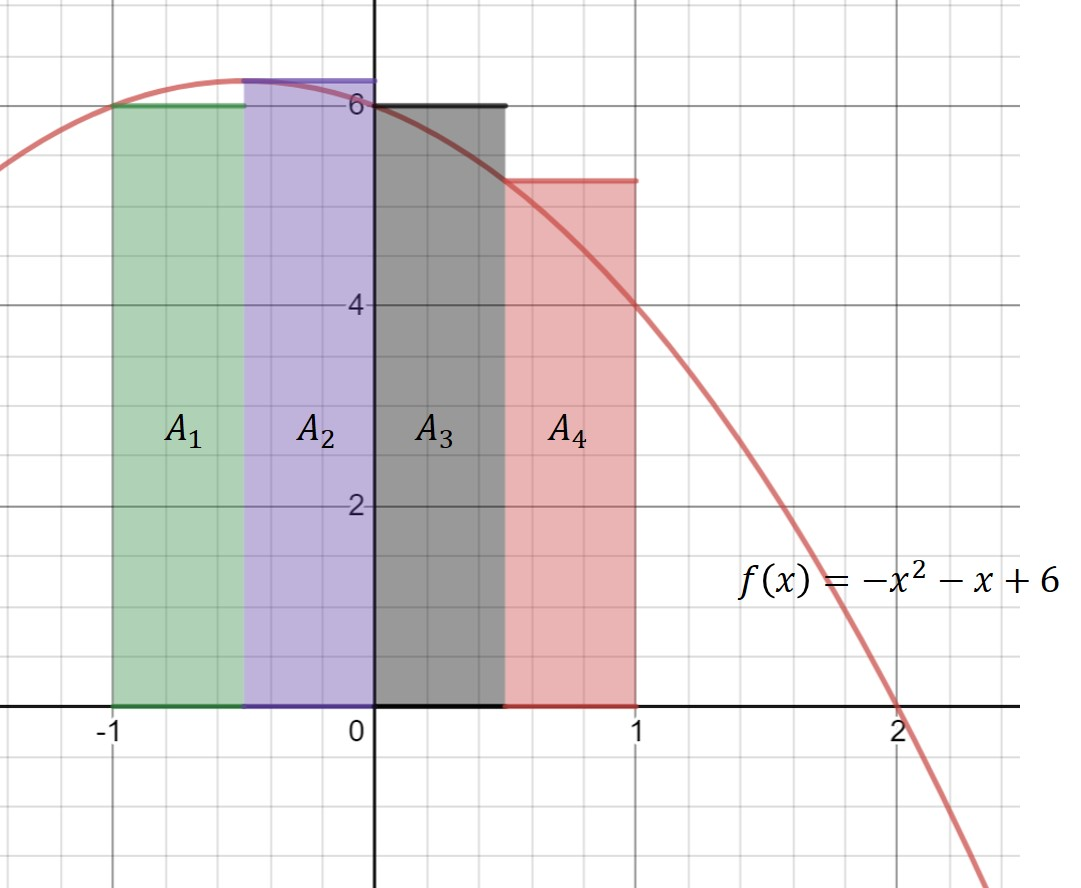
\includegraphics[height=1in]{240test3image1.jpg}

\end{image}
Find the exact area of each rectangle.
$$A_1=\answer{3},\quad A_2=\answer{3.125},\quad A_3=\answer{3},\quad A_4=\answer{2.625}$$

Estimate the total area under the curve.
$$\mbox{Total Area Under the Curve }\approx \Sigma_{i=1}^{i=4}A_i=\answer{11.75}$$
\item
Set up and evaluate a definite integral to find the exact area under the curve $y=f(x)$ on the interval $[-1,1]$.
$$\int_{\answer{-1}}^{\answer{1}}\answer{-x^2-x+6}\,dx=\answer[tolerance=0.1]{11.33}$$
\end{enumerate}
\end{problem}

\begin{problem}\label{prob:mth240exam3prob2}
Evaluate the indefinite integral.
  \begin{enumerate}
\item
$\int 5x^2+\sqrt{x}\,dx=\answer{\frac{5}{3}x^3+\frac{2}{3}x^{1.5}}+C$

\item
$\int e^x+\cos x\, dx=\answer{e^x+\sin x}+C$

\item
$\int \frac{x+x^2}{x}\,dx=\answer{x+0.5x^2}+C$
  \end{enumerate}
\end{problem}

\begin{problem}\label{prob:mth240exam3prob3}
Evaluate the definite integral.  Enter exact values; no decimal approximations.
  \begin{enumerate}
\item
$\int_1^5 4x+1\, dx=\answer{52}$

\item
$\int_{-\pi}^{\pi} \sin x\, dx=\answer{0}$

\item
$\int_{-1}^1 x^2\, dx=\answer{\frac{2}{3}}$

  \end{enumerate}

\end{problem}

\begin{problem}\label{prob:mth240exam3prob4}
Find the total area bounded by the curve given by $f(x)=\sin x$ on the interval $[0, 2\pi]$.

Total geometric area (positive number): $\answer{4}$
\end{problem}


\end{document} 